\documentclass[12pt,a4paper]{report}

\usepackage[T1]{fontenc}
\usepackage{amsmath}
\usepackage{amssymb}
\usepackage{microtype}
\usepackage[top=1in,bottom=1in,left=1.25in,right=1in]{geometry}
\renewcommand{\rmdefault}{ptm}
\usepackage{setspace}
\usepackage{graphicx}
\usepackage{tabularx}
\usepackage{longtable}
\usepackage{array}
\usepackage{float}
\usepackage{caption}
\usepackage{hyperref}
\usepackage{fancyhdr}
\usepackage{titlesec}
\usepackage{xcolor}
\usepackage{listings}

\lstset{
  basicstyle=\small\ttfamily,
  breaklines=true,
  showstringspaces=false,
  keywordstyle=\color{blue},
  commentstyle=\color{gray},
  stringstyle=\color{red!70!black},
  numbers=left,
  numberstyle=\tiny,
  columns=flexible,
  frame=single,
  rulecolor=\color{black!30}
}

\onehalfspacing
\setlength{\parindent}{0pt}
\setlength{\parskip}{6pt}

% Heading formatting per syllabus: chapter 16pt (centred), section 14pt,
% subsection 12pt, all bold.
\titleformat{\chapter}[display]
  {\normalfont\fontsize{16}{19}\bfseries\centering}
  {\MakeUppercase{\chaptertitlename}\ \thechapter}
  {0.6em}
  {}
\titlespacing*{\chapter}{0pt}{0pt}{24pt}
\titleformat{\section}
  {\normalfont\fontsize{14}{17}\bfseries}{\thesection}{1em}{}
\titleformat{\subsection}
  {\normalfont\fontsize{12}{15}\bfseries}{\thesubsection}{1em}{}
\titleformat{\subsubsection}
  {\normalfont\fontsize{12}{15}\bfseries}{\thesubsubsection}{1em}{}

% Captions: bold, 12pt, centred (figures below, tables above).
\captionsetup{font=bf,labelsep=colon,justification=centering,singlelinecheck=false}
\renewcommand{\contentsname}{Table of Contents}
\renewcommand{\listtablename}{List of Tables}
\renewcommand{\listfigurename}{List of Figures}
\renewcommand{\bibname}{References}

\pagestyle{fancy}
\fancyhf{}
\fancyfoot[C]{\thepage}
\renewcommand{\headrulewidth}{0pt}
\fancypagestyle{plain}{\fancyhf{}\fancyfoot[C]{\thepage}\renewcommand{\headrulewidth}{0pt}}

\hypersetup{
  colorlinks=true,
  linkcolor=black,
  citecolor=black,
  urlcolor=blue,
  pdftitle={CampusEase Final Year Project Report},
  pdfauthor={Bhupendra Malla}
}

\newcommand{\code}[1]{\texttt{\small #1}}

\begin{document}

\hypersetup{pageanchor=false}

% =====================================================================
% TITLE PAGE
% =====================================================================
\begin{titlepage}
\begin{center}

\textbf{\fontsize{14}{17}\selectfont Lincoln University College}\\[4pt]
\textbf{\fontsize{12}{15}\selectfont Faculty of Computer Science and Multimedia}\\[26pt]

\textbf{\fontsize{16}{19}\selectfont CampusEase: A Web-Based College Automation\\
System for Academic and Administrative Management}\\[24pt]

\textbf{\fontsize{14}{17}\selectfont FINAL YEAR PROJECT REPORT}\\[10pt]
\fontsize{12}{15}\selectfont
Submitted to\\[4pt]
Department of Information Technology\\
Phoenix College of Management\\
Maitidevi, Kathmandu\\[20pt]

In partial fulfillment of the requirements for the degree of\\
\textbf{Bachelor in Information Technology (BIT)}\\[24pt]

Submitted by\\[8pt]
\textbf{Bhupendra Malla}\\
BIT 8th Semester\\
University ID: LC0003001648\\[18pt]

Under the Supervision of\\[4pt]
\textbf{Mr. Saishab Bhattarai}\\
Project Supervisor\\[18pt]

\vfill
\textbf{May, 2026}

\end{center}
\end{titlepage}

\clearpage
\hypersetup{pageanchor=true}
\pagenumbering{roman}

% =====================================================================
% LETTER OF APPROVAL
% =====================================================================
\begin{center}

\includegraphics[width=3.4cm]{figures/university_logo.png}\\[8pt]
\textbf{\fontsize{14}{17}\selectfont Lincoln University College}\\
{\fontsize{12}{14}\selectfont Faculty of Computer Science and Multimedia}\\
{\fontsize{12}{14}\selectfont Phoenix College of Management, Maitidevi, Kathmandu}\\[14pt]
\textbf{\fontsize{16}{19}\selectfont LETTER OF APPROVAL}
\end{center}
\addcontentsline{toc}{chapter}{Letter of Approval}
\vspace{0.6cm}

This is to certify that this project report titled ``CampusEase: A Web-Based College Automation System for Academic and Administrative Management'' prepared and submitted by Bhupendra Malla (University ID: LC0003001648) in partial fulfillment of the requirements for the degree of Bachelor in Information Technology (BIT) has been reviewed and approved.

The project has been carried out under supervision and meets the academic standards required by the Department of Information Technology, Phoenix College of Management.

\vspace{2.2cm}

\noindent
\begin{tabular}{p{6.2cm}p{6.2cm}}
\underline{\hspace{5cm}} & \underline{\hspace{5cm}} \\
\textbf{Mr. Saishab Bhattarai} & \textbf{Project Coordinator} \\
Project Supervisor & Department of Information Technology \\
Department of Information Technology & Phoenix College of Management \\[1.6cm]
\underline{\hspace{5cm}} & \underline{\hspace{5cm}} \\
\textbf{Internal Examiner} & \textbf{External Examiner} \\
\end{tabular}

\clearpage

% =====================================================================
% SUPERVISOR'S CERTIFICATE
% =====================================================================
\begin{center}\textbf{\fontsize{16}{19}\selectfont SUPERVISOR'S CERTIFICATE}\end{center}
\addcontentsline{toc}{chapter}{Supervisor's Certificate}
\vspace{0.6cm}

This is to certify that the student Bhupendra Malla has completed the Bachelor in Information Technology Final Year Project titled ``CampusEase: A Web-Based College Automation System for Academic and Administrative Management'' under the supervision of Mr. Saishab Bhattarai at Lincoln University College, Faculty of Computer Science and Multimedia.

The student has independently designed and implemented a working software prototype, conducted testing, and documented the system according to academic standards. To the best of my knowledge, the work presented in this report is original and has not been submitted elsewhere for the award of any degree.

I recommend this project report for evaluation.

\vspace{2.5cm}

\noindent
Signature: \underline{\hspace{5.5cm}}\\[0.4cm]
\textbf{Mr. Saishab Bhattarai}\\
Project Supervisor\\
Department of Information Technology\\
Phoenix College of Management

\clearpage

% =====================================================================
% ACKNOWLEDGEMENT
% =====================================================================
\begin{center}\textbf{\fontsize{16}{19}\selectfont ACKNOWLEDGEMENT}\end{center}
\addcontentsline{toc}{chapter}{Acknowledgement}
\vspace{0.6cm}

I would like to express my sincere gratitude to all those who contributed directly and indirectly to the successful completion of this project. Their guidance, encouragement, and continuous support have been invaluable throughout the entire course of this work.

First and foremost, I would like to express my profound gratitude to the Principal of Phoenix College of Management, Prof. Dr. Fatta Bahadur KC, for his inspiring leadership, academic guidance, and continuous encouragement in fostering an environment dedicated to learning, research, and innovation.

I would also like to extend my heartfelt appreciation to my project supervisor, Mr. Saishab Bhattarai, for his invaluable guidance, constructive feedback, encouragement, and continuous support throughout the development of this project. His expertise, patience, and insightful suggestions greatly contributed to the successful completion of this work.

Furthermore, I am deeply thankful to the Department of Information Technology at Phoenix College of Management for providing the necessary academic environment, institutional support, resources, and facilities required for the successful execution of this project.

I would also like to acknowledge the valuable support and encouragement provided by the faculty members, whose suggestions and assistance played a significant role during the course of this work.

Finally, I express my deepest gratitude to my family and friends for their unwavering support, motivation, patience, and encouragement throughout this journey. Their constant belief in me provided the strength and determination necessary to accomplish this project successfully.

\vspace{1cm}
\noindent
\textbf{Bhupendra Malla}\\
BIT 8th Semester\\
University ID: LC0003001648

\clearpage

% =====================================================================
% ABSTRACT
% =====================================================================
\begin{center}\textbf{\fontsize{16}{19}\selectfont ABSTRACT}\end{center}
\addcontentsline{toc}{chapter}{Abstract}
\vspace{0.6cm}

Colleges run on a large number of overlapping manual processes: enrollment, attendance, assignments, examinations, fee collection, scheduling, and day-to-day communication between students, faculty, and administrative staff. Handling these on paper and across disconnected tools is slow, error-prone, and difficult to track. CampusEase is a web-based college automation system that brings these activities together on a single platform. It provides role-based access for students, faculty, secretaries, and administrators; supports subject enrollment and class scheduling; records attendance manually, through a one-time password, or through face recognition; manages assignment distribution and submission, internal marks entry, and automatic internal-marks calculation; and integrates online fee payment through the Khalti gateway with an administrative approval workflow. Real-time messaging, discussion forums, events, clubs, a job-and-CV portal, sponsorship requests, and digital ID-card generation are also included. The system is built with an Angular single-page frontend, a Node.js and Express REST API with Socket.io for real-time features, and a MongoDB database accessed through the Mongoose object-document mapper, with JWT authentication and bcrypt password hashing. The result is a reliable, easy-to-use platform that reduces administrative workload, minimizes errors, and improves transparency and communication across the academic community.

\vspace{0.6cm}
\noindent\textbf{Keywords:} College Automation, Student Information System, Role-Based Access Control, Face Recognition Attendance, Online Fee Payment, Real-Time Communication.

\clearpage

% =====================================================================
% TABLE OF CONTENTS / LISTS
% =====================================================================
\tableofcontents
\clearpage
\addcontentsline{toc}{chapter}{List of Figures}
\listoffigures
\clearpage
\addcontentsline{toc}{chapter}{List of Tables}
\listoftables
\clearpage

% =====================================================================
% LIST OF ABBREVIATIONS
% =====================================================================
\begin{center}\textbf{\fontsize{16}{19}\selectfont LIST OF ABBREVIATIONS}\end{center}
\addcontentsline{toc}{chapter}{List of Abbreviations}
\vspace{0.6cm}

\begin{longtable}{p{3cm}p{10.5cm}}
\textbf{Abbreviation} & \textbf{Full Form} \\[4pt]
\endfirsthead
\textbf{Abbreviation} & \textbf{Full Form} \\[4pt]
\endhead
API & Application Programming Interface \\
BIT & Bachelor in Information Technology \\
CRUD & Create, Read, Update, Delete \\
CSS & Cascading Style Sheets \\
DFD & Data Flow Diagram \\
ER & Entity Relationship \\
ERP & Enterprise Resource Planning \\
HTTP & Hypertext Transfer Protocol \\
JSON & JavaScript Object Notation \\
JWT & JSON Web Token \\
LMS & Learning Management System \\
NoSQL & Not Only Structured Query Language \\
ODM & Object Document Mapper \\
OTP & One-Time Password \\
RBAC & Role-Based Access Control \\
REST & Representational State Transfer \\
SIS & Student Information System \\
SMTP & Simple Mail Transfer Protocol \\
SPA & Single-Page Application \\
UI & User Interface \\
UML & Unified Modeling Language \\
VCS & Version Control System \\
\end{longtable}

\clearpage
\pagenumbering{arabic}

% =====================================================================
% CHAPTER 1: INTRODUCTION
% =====================================================================
\chapter{Introduction}

\section{Introduction}

Educational institutions handle an enormous amount of routine work every day. Students enroll in subjects, attend classes, submit assignments, sit examinations, and pay fees. Faculty members prepare schedules, take attendance, distribute and grade assignments, and record marks. Administrative staff manage accounts, approve payments, maintain departments, organize events, and issue documents such as identity cards. Traditionally, most of this work is done manually, on paper, or across a collection of disconnected applications and spreadsheets.

This manual, fragmented approach is slow and error-prone. Records are duplicated or lost, attendance and marks are tedious to compile, fee tracking is hard to reconcile, and communication between students, faculty, and staff relies on notice boards and informal channels. As colleges grow and as students increasingly expect digital, mobile-friendly services, these problems become more pronounced.

A college automation system addresses this by bringing the core academic and administrative activities of an institution onto a single, integrated platform. Instead of separate, manual processes, a well-designed system gives each kind of user a tailored interface, keeps a single authoritative copy of every record, automates repetitive calculations, and enables instant communication. The benefits are reduced workload, fewer errors, faster access to information, and greater transparency for everyone involved.

CampusEase is such a system. It is a web-based platform that unifies enrollment, scheduling, attendance, assignments, examinations and marks, fee payment, and communication, with role-based access for students, faculty, secretaries, and administrators. It adds modern conveniences such as face-recognition attendance, online fee payment through a local payment gateway, real-time messaging, and digital ID-card generation, all behind a clean interface that requires no special technical training to use.

\section{Problem Statement}

Most colleges still rely on manual or loosely connected processes to run their academic and administrative operations. This creates several concrete problems that CampusEase is designed to solve:

\begin{itemize}
    \item \textbf{Fragmented information.} Student records, attendance, marks, fees, and communication are spread across paper registers, spreadsheets, and unrelated tools, with no single source of truth.
    \item \textbf{Manual, repetitive work.} Taking attendance, compiling internal marks, reconciling fee payments, and preparing reports by hand is slow and consumes staff and faculty time that could be better spent.
    \item \textbf{Error and inconsistency.} Re-entering the same data in multiple places leads to mistakes, and there is often no reliable audit trail of who changed what.
    \item \textbf{Weak communication.} Important information reaches students through notice boards or third-party messaging, so updates are easy to miss and hard to track.
    \item \textbf{Limited access control.} Without a structured permission model, it is difficult to ensure that each user, from a student to a finance officer, sees and does only what their role allows.
\end{itemize}

There is a clear need for an integrated, role-aware web platform that centralizes academic and administrative data, automates routine tasks such as attendance and marks calculation, supports secure online fee payment, and provides direct, real-time communication, all through a simple interface.

\section{Objectives}

\subsection{General Objective}

To design and develop a web-based college automation system that centralizes academic and administrative operations and provides role-based, automated services to students, faculty, and administrative staff.

\subsection{Specific Objectives}

\begin{itemize}
    \item To study existing college automation, student information, and learning management systems and identify their limitations.
    \item To design a role-based access control model covering students, faculty, secretaries, and administrators.
    \item To implement subject enrollment, class scheduling, and academic-record management.
    \item To provide multiple attendance methods, including manual, one-time-password, and face-recognition attendance.
    \item To automate assignment distribution and submission, marks entry, and internal-marks calculation.
    \item To integrate secure online fee payment through the Khalti gateway with an administrative approval workflow.
    \item To enable real-time communication through messaging, discussion forums, events, and clubs.
    \item To ensure the system is secure, usable, and accessible to users with basic technical knowledge.
\end{itemize}

\section{Significance of the Study}

CampusEase demonstrates how a single, well-structured web application can replace a collection of manual and disconnected processes in a college. For students, it offers a single portal for enrollment, attendance, assignments, marks, fees, and communication. For faculty, it automates scheduling, attendance, and marks-related tasks. For administrative staff, it provides structured user management, fee approval, and reporting. Beyond the institution it serves, the project is a practical case study in building a real, multi-role web system with modern technologies, secure authentication, real-time features, and third-party payment integration, and is therefore valuable both as a deployable product and as an academic learning outcome.

\section{Scope and Limitation}

\subsection{Scope}

CampusEase is an integrated college automation platform. Its scope includes:

\begin{itemize}
    \item Role-based registration and authentication for students, faculty, secretaries, and administrators, with email verification and one-time-password support.
    \item Subject enrollment using enrollment keys, class scheduling, and academic-record management.
    \item Attendance recording through manual entry, one-time password, and face recognition.
    \item Assignment distribution and submission, marks entry, and automatic internal-marks calculation from assignment and attendance scores.
    \item Online fee payment through the Khalti gateway, with payment status tracking and administrative approval.
    \item Real-time one-to-one messaging, discussion forums, events, and club membership.
    \item A job-and-CV portal, sponsorship requests, digital ID-card generation, feedback collection, and dashboards.
\end{itemize}

\subsection{Limitation}

\begin{itemize}
    \item The system is a web application intended for use within a single institution; it is not a multi-tenant product serving many colleges from one deployment.
    \item Face-recognition attendance depends on adequate lighting and a working camera, and is intended as a convenience method alongside manual and one-time-password attendance rather than a biometric-grade security control.
    \item Online payment is integrated with the Khalti gateway; other payment methods are recorded but processed manually by staff.
    \item The current deployment uses a single MongoDB instance suitable for an institution-scale workload and academic demonstration rather than very large, high-concurrency, multi-campus environments.
    \item Authentication uses JWT with bcrypt-hashed passwords appropriate for the project; a large production deployment would add measures such as refresh-token rotation and centralized session management.
\end{itemize}

\section{Development Methodology}

The project was developed using an Agile methodology based on short, iterative sprints. Because CampusEase is made up of many distinct but related modules (authentication, enrollment, attendance, assignments, marks, fees, communication, and administration), an incremental, feature-by-feature approach was a natural fit. Each sprint delivered one or more working modules: requirements were refined, the data model and API endpoints were built on the backend, the corresponding Angular screens were developed, and the feature was tested before moving on. The role-based access model and the user data model were built early because almost every later feature depends on them. Version control with Git and GitHub was used throughout, allowing changes to be tracked incrementally and modules to be integrated continuously. This iterative style made it possible to absorb feedback and add modules without disrupting features already completed.

\section{Report Organization}

The remainder of this report is organized as follows. Chapter 2 reviews college automation concepts and existing systems and positions CampusEase against them. Chapter 3 presents the system analysis and design, including the feasibility study, requirements, use-case and data models, data flow diagrams, and system design. Chapter 4 describes the implementation of each module and the testing approach and results. Chapter 5 concludes the report and discusses lessons learned and future enhancements.

% =====================================================================
% CHAPTER 2: BACKGROUND STUDY AND LITERATURE REVIEW
% =====================================================================
\chapter{Background Study and Literature Review}

\section{Background Study}

\textbf{College Automation and Student Information Systems.}
A college automation system, sometimes called a campus management or student information system (SIS), is software that digitizes and integrates an institution's academic and administrative processes. Rather than maintaining separate records for admissions, attendance, examinations, and finance, such a system keeps one connected set of data and exposes it through role-specific interfaces. The expected benefits, widely reported in the literature, are reduced manual effort, fewer data-entry errors, faster reporting, and improved communication among stakeholders.

\textbf{Learning Management and ERP Systems.}
Two related families of systems are relevant. Learning Management Systems (LMS) such as Moodle and Google Classroom focus on the teaching and learning workflow: distributing course material, collecting assignments, and grading. Enterprise Resource Planning (ERP) systems for education go further, covering finance, human resources, and operations alongside academics, but they are large, costly, and aimed at big institutions. CampusEase sits between these: it covers the academic workflow like an LMS while also handling administrative tasks such as fee payment, user management, and document issuance, but it remains lightweight and tailored to a single college.

\textbf{Web Application Architecture.}
Modern web applications are commonly built as a single-page application (SPA) frontend communicating with a backend API over HTTP, often complemented by WebSocket connections for real-time features. CampusEase follows this pattern with an Angular SPA, an Express REST API, and Socket.io for live messaging. Data is stored in a NoSQL document database, MongoDB, accessed through the Mongoose object-document mapper, which suits the varied and evolving document shapes of a college's records.

\section{Literature Review}

Several established systems address parts of the same problem space:

\begin{itemize}
    \item \textbf{Google Classroom}~\cite{googleclassroom} is a free, widely used platform for distributing material, posting assignments, and grading. It is simple and reliable but is focused on the classroom workflow and does not handle administrative concerns such as fee payment, attendance registers, or institutional user management.
    \item \textbf{Moodle}~\cite{moodle} is a mature, open-source LMS that is highly configurable and extensible through plugins. It is powerful for course delivery, but it is heavy to host and administer and is not designed as an end-to-end college administration system.
    \item \textbf{Microsoft Teams for Education} combines communication, meetings, and assignment features. It excels at communication and collaboration but, like the others, is not a complete academic-plus-administrative platform and depends on the wider Microsoft ecosystem.
    \item \textbf{Commercial campus ERPs} provide comprehensive coverage of academics, finance, and operations, but they are expensive, complex to deploy, and far larger than a single college usually needs.
\end{itemize}

Table~\ref{tab:comparison} compares these systems against the needs CampusEase targets.

\begin{table}[H]
\centering
\caption{Comparison of existing systems with the needs CampusEase targets.}
\label{tab:comparison}
\small
\begin{tabular}{|p{2.8cm}|p{2.3cm}|p{2.1cm}|p{2.3cm}|p{2.3cm}|}
\hline
\textbf{Criterion} & \textbf{Google Classroom} & \textbf{Moodle} & \textbf{Campus ERP} & \textbf{CampusEase} \\
\hline
Cost & Free & Free (self-host) & Costly & Free \\
\hline
Setup effort & Low & High & High & Low \\
\hline
Academic workflow & Yes & Yes & Yes & Yes \\
\hline
Administration (fees, users) & No & Partial & Yes & Yes \\
\hline
Attendance register & No & Plugin & Yes & Yes (manual/OTP/face) \\
\hline
Online fee payment & No & No & Yes & Yes (Khalti) \\
\hline
Real-time messaging & Limited & Limited & Varies & Yes (Socket.io) \\
\hline
\end{tabular}
\end{table}

The common limitation is clear: learning management tools cover teaching but not administration, while full ERPs cover everything but are costly and complex. Neither is well matched to a single college that wants both academic and administrative automation in one affordable, easy-to-run package. CampusEase addresses this gap by combining an LMS-style academic workflow with administrative features, role-based access for every type of user, modern conveniences such as face-recognition attendance and online payment, and real-time communication, all on a lightweight stack that a small institution can operate without specialist staff.

% =====================================================================
% CHAPTER 3: SYSTEM ANALYSIS AND DESIGN
% =====================================================================
\chapter{System Analysis and Design}

\section{System Analysis}

CampusEase is organized around the roles of the people who use it and the tasks each role performs. At a high level the system supports four broad activities: (1) \textbf{authentication and authorization}, where users register, verify their identity, sign in, and are granted role-specific access; (2) \textbf{academic management}, covering enrollment, scheduling, attendance, assignments, marks, and records; (3) \textbf{financial and administrative management}, covering fee payment and approval, user and department management, ID cards, and reporting; and (4) \textbf{communication and engagement}, covering real-time messaging, discussion forums, events, and clubs. Each activity is exposed through REST API endpoints on the backend and corresponding screens on the Angular frontend, and is restricted to the roles permitted to use it.

\subsection{Requirement Analysis}

\subsubsection{Functional Requirements}

Table~\ref{tab:fr} lists the functional requirements of CampusEase. The corresponding actor interactions are modelled by the use-case diagram in Figure~\ref{fig:usecase}.

\begin{longtable}{|p{1.3cm}|p{4cm}|p{7.5cm}|}
\caption{Functional requirements of CampusEase.}
\label{tab:fr}\\
\hline
\textbf{ID} & \textbf{Requirement} & \textbf{Description} \\
\hline
\endfirsthead
\hline
\textbf{ID} & \textbf{Requirement} & \textbf{Description} \\
\hline
\endhead
FR-01 & Registration \& verification & The system shall allow a user to register and verify the account by email, and shall set a password securely. \\
\hline
FR-02 & Authentication & The system shall allow a registered user to log in and shall reject invalid credentials. \\
\hline
FR-03 & Role-based access & The system shall grant access to features according to the user's role (student, faculty, secretary, administrator, and related staff roles). \\
\hline
FR-04 & Subject enrollment & The system shall allow a student to enroll in subjects for a semester using an enrollment key. \\
\hline
FR-05 & Class scheduling & The system shall allow faculty or staff to create, update, and view class schedules. \\
\hline
FR-06 & Attendance & The system shall record attendance through manual entry, one-time password, and face recognition. \\
\hline
FR-07 & Assignments & The system shall allow faculty to post assignments and students to submit answers with file uploads. \\
\hline
FR-08 & Marks entry & The system shall allow faculty to enter and update student marks. \\
\hline
FR-09 & Internal-marks calculation & The system shall compute internal marks automatically from assignment and attendance scores. \\
\hline
FR-10 & Fee payment & The system shall allow a student to pay fees online through the Khalti gateway and shall record the payment. \\
\hline
FR-11 & Fee approval & The system shall allow an administrator or finance officer to approve or reject fee payments. \\
\hline
FR-12 & Messaging & The system shall provide real-time one-to-one messaging between users. \\
\hline
FR-13 & Discussion \& engagement & The system shall support discussion forums, events, and club membership. \\
\hline
FR-14 & Career services & The system shall allow CV submission and job-vacancy posting, and sponsorship requests. \\
\hline
FR-15 & ID cards \& reports & The system shall generate digital ID cards and provide administrative dashboards and reports. \\
\hline
FR-16 & User management & The system shall allow authorized staff to create, update, and delete user accounts. \\
\hline
\end{longtable}

\subsubsection{Non-functional Requirements}

Table~\ref{tab:nfr} lists the non-functional requirements.

\begin{longtable}{|p{1.5cm}|p{3.5cm}|p{8cm}|}
\caption{Non-functional requirements of CampusEase.}
\label{tab:nfr}\\
\hline
\textbf{ID} & \textbf{Requirement} & \textbf{Description} \\
\hline
\endfirsthead
\hline
\textbf{ID} & \textbf{Requirement} & \textbf{Description} \\
\hline
\endhead
NFR-01 & Performance & The system shall respond to typical requests within a couple of seconds and deliver messages in real time. \\
\hline
NFR-02 & Usability & The interface shall be intuitive and operable by a user with basic technical knowledge. \\
\hline
NFR-03 & Security & The system shall hash passwords, authenticate requests with JSON Web Tokens, and enforce role-based access. \\
\hline
NFR-04 & Reliability & The system shall handle invalid input and unavailable external services gracefully, without crashing. \\
\hline
NFR-05 & Maintainability & The codebase shall be modular, separating routes, models, and services on the backend and components and services on the frontend. \\
\hline
NFR-06 & Portability & The system shall run on any platform with a Node.js runtime and a MongoDB instance. \\
\hline
NFR-07 & Scalability & The system shall support an institution-scale number of users and allow modules to be added without major redesign. \\
\hline
\end{longtable}

\subsection{Feasibility Study}

\textbf{Technical Feasibility.}
The system is technically feasible. It is built with mature, widely used web technologies: Angular for the frontend, Node.js and Express for the backend API, Socket.io for real-time messaging, and MongoDB with Mongoose for storage. Authentication uses JSON Web Tokens and bcrypt password hashing, and payment uses the publicly documented Khalti gateway. All core libraries are open-source and run on commodity hardware without specialized infrastructure.

\textbf{Operational Feasibility.}
The system is operationally feasible. It is designed for everyday users, students, faculty, and administrative staff, with role-specific interfaces that guide each user through their tasks. No command-line use or technical configuration is required to operate the system once it is deployed.

\textbf{Economic Feasibility.}
The system is economically feasible. The frameworks, database, and libraries are open-source, and the Khalti gateway is a standard local payment service. The platform can be hosted on modest, low-cost infrastructure, so both development and operational costs are minimal.

\textbf{Schedule Feasibility.}
The project was planned across an iterative, multi-sprint schedule covering requirement analysis and design, the authentication and role model, the academic modules, the financial and communication modules, and finally integration, testing, and documentation. Building the system module by module allowed a complete, working platform to be delivered within the available time.

\subsection{Use-Case Modelling}

The use-case diagram in Figure~\ref{fig:usecase} shows the main actors, students, faculty, and administrators or secretaries, and the use cases each performs, together with the external Khalti payment gateway and email service. Registration includes email verification, paying fees includes a call to the Khalti gateway and can be extended by an administrative approval step, and submitting an assignment relates to the faculty task of posting and grading it.

\begin{figure}[H]
    \centering
    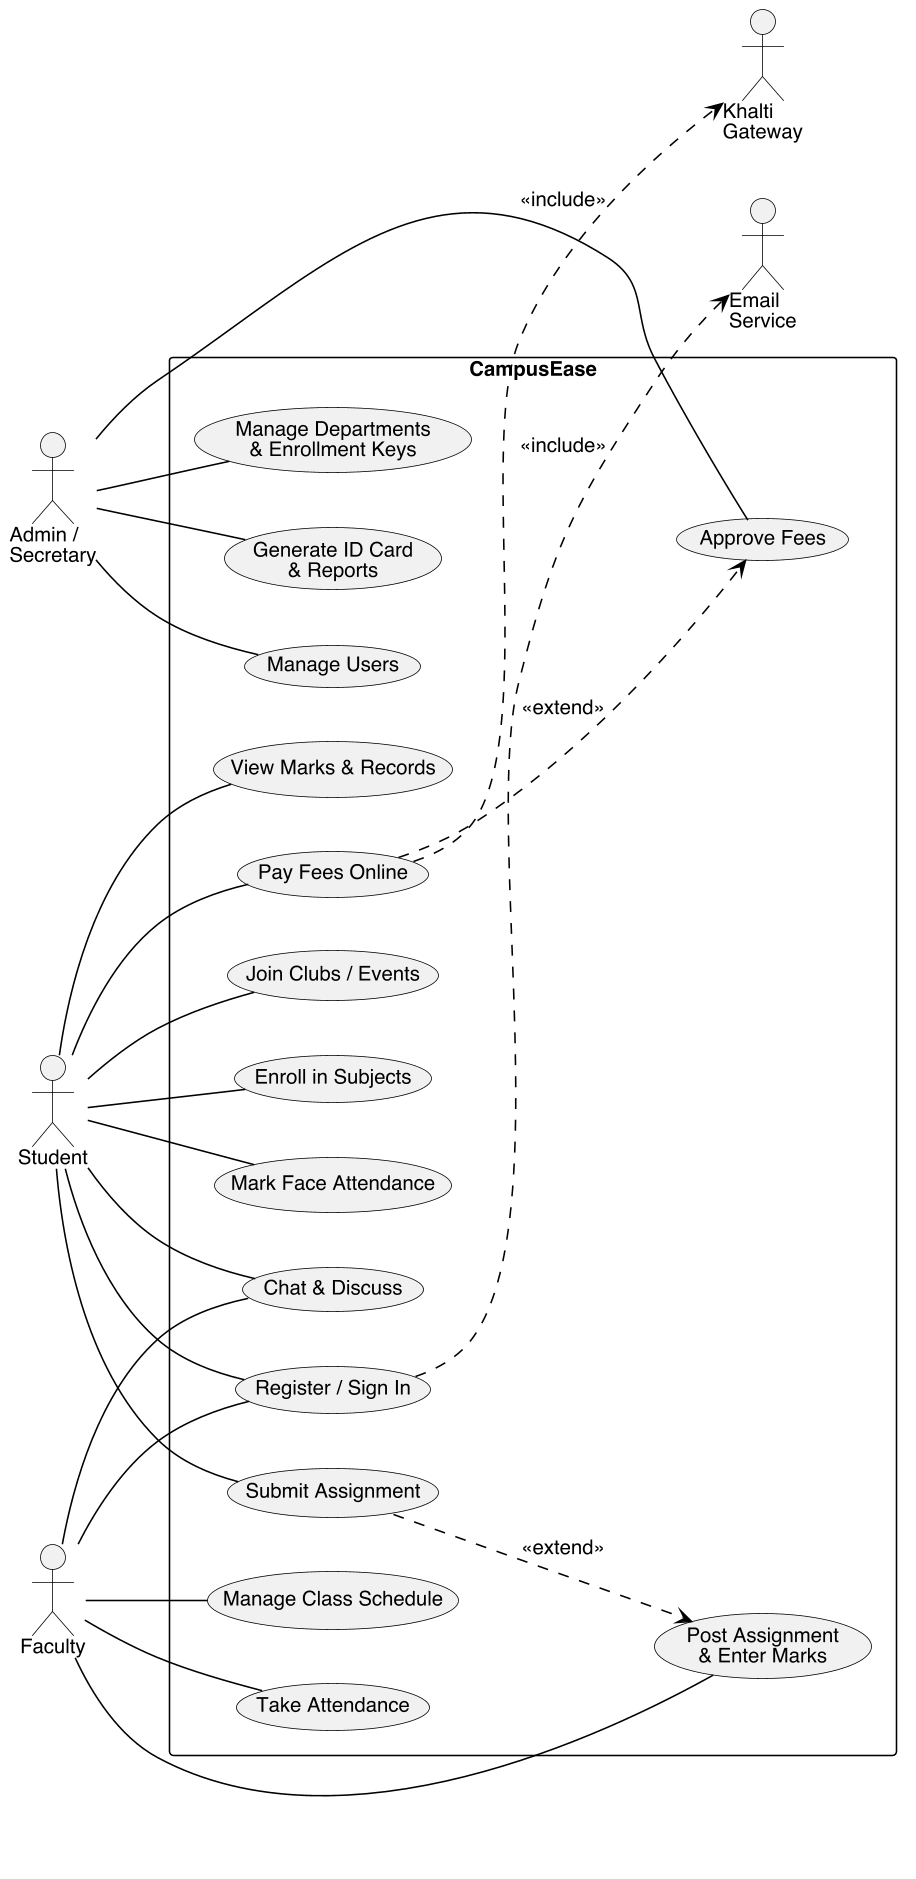
\includegraphics[width=0.72\textwidth,height=0.82\textheight,keepaspectratio]{figures/use_case_diagram.png}
    \caption{Use-case diagram of CampusEase.}
    \label{fig:usecase}
\end{figure}

\subsection{Data Modelling: Entity-Relationship Diagram}

The data model is stored as MongoDB collections accessed through Mongoose. The core entities are \code{User}, \code{EnrollmentSubjects}, \code{Attendance}, \code{GiveAssignment}, \code{AnswerAssignment}, \code{MarksEntry}, \code{Fee}, and \code{Message}. A user owns many attendance records, assignment submissions, fee payments, marks, and messages; an enrollment groups the assignments for its subjects; and each posted assignment is answered by many submissions. Figure~\ref{fig:er} shows the entity-relationship diagram.

\begin{figure}[H]
    \centering
    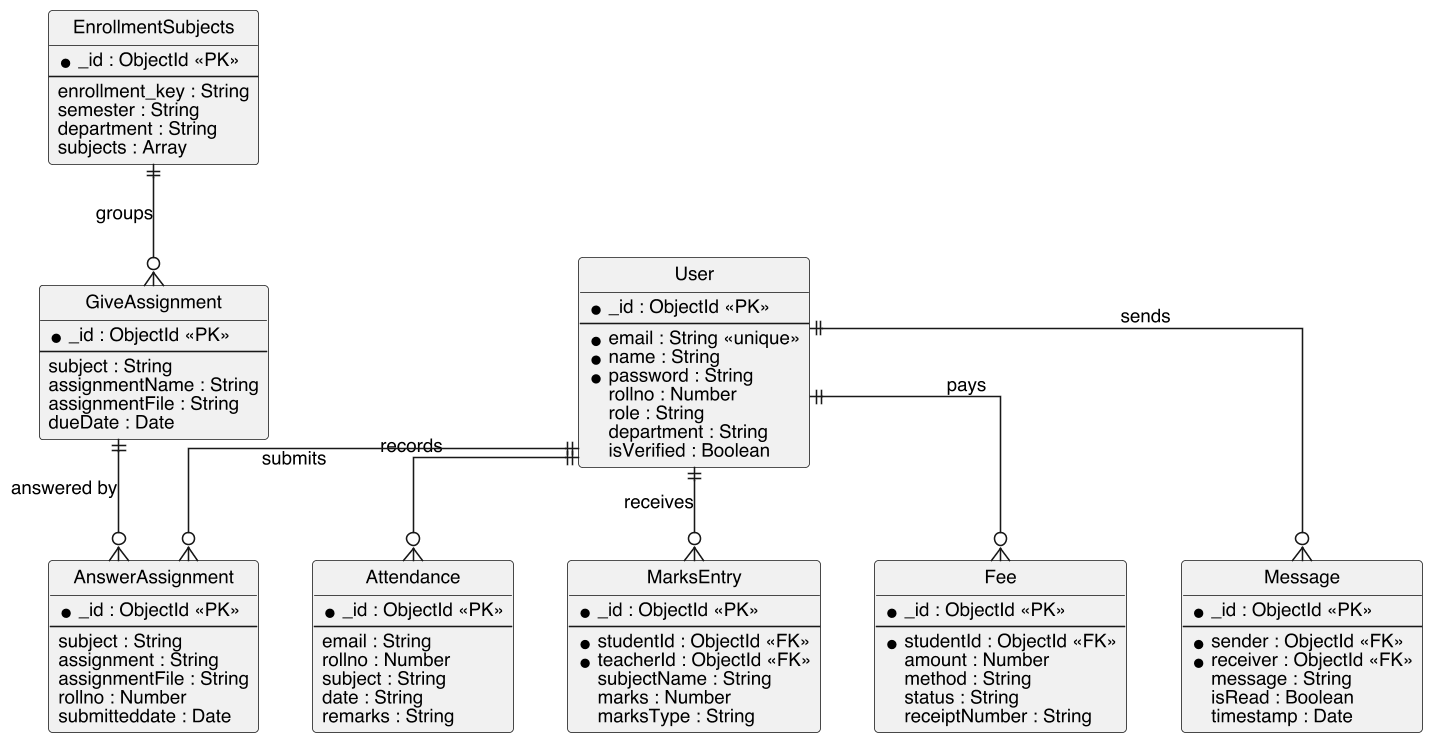
\includegraphics[width=0.92\textwidth,height=0.80\textheight,keepaspectratio]{figures/er_diagram.png}
    \caption{Entity-relationship diagram of CampusEase.}
    \label{fig:er}
\end{figure}

\subsection{Process Modelling: Data Flow Diagrams}

The context-level (Level 0) data flow diagram in Figure~\ref{fig:dfd0} shows CampusEase as a single process exchanging data with its users, the Khalti payment gateway, and the email service.

\begin{figure}[H]
    \centering
    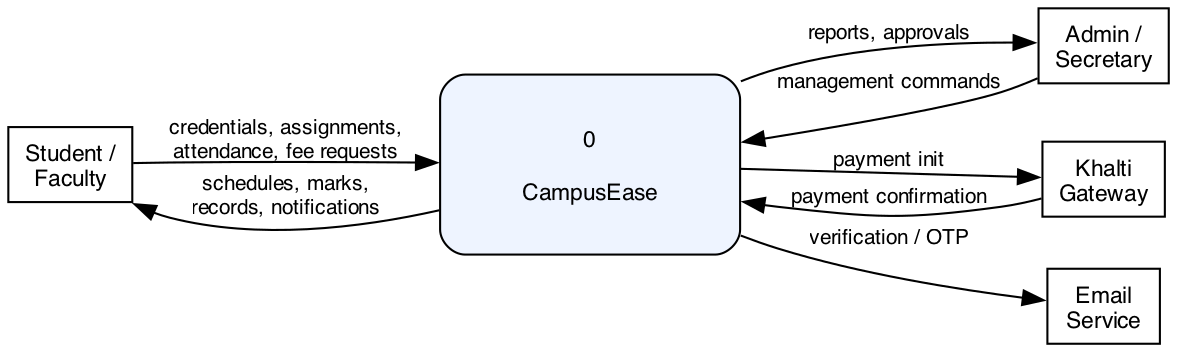
\includegraphics[width=0.95\textwidth,height=0.5\textheight,keepaspectratio]{figures/dfd_level0.png}
    \caption{Context-level (Level 0) data flow diagram.}
    \label{fig:dfd0}
\end{figure}

The Level 1 data flow diagram in Figure~\ref{fig:dfd1} decomposes the system into six processes, authenticate and authorize, manage academics, record attendance, manage assignments and marks, process fee payment, and communication and engagement, communicating through six data stores.

\begin{figure}[H]
    \centering
    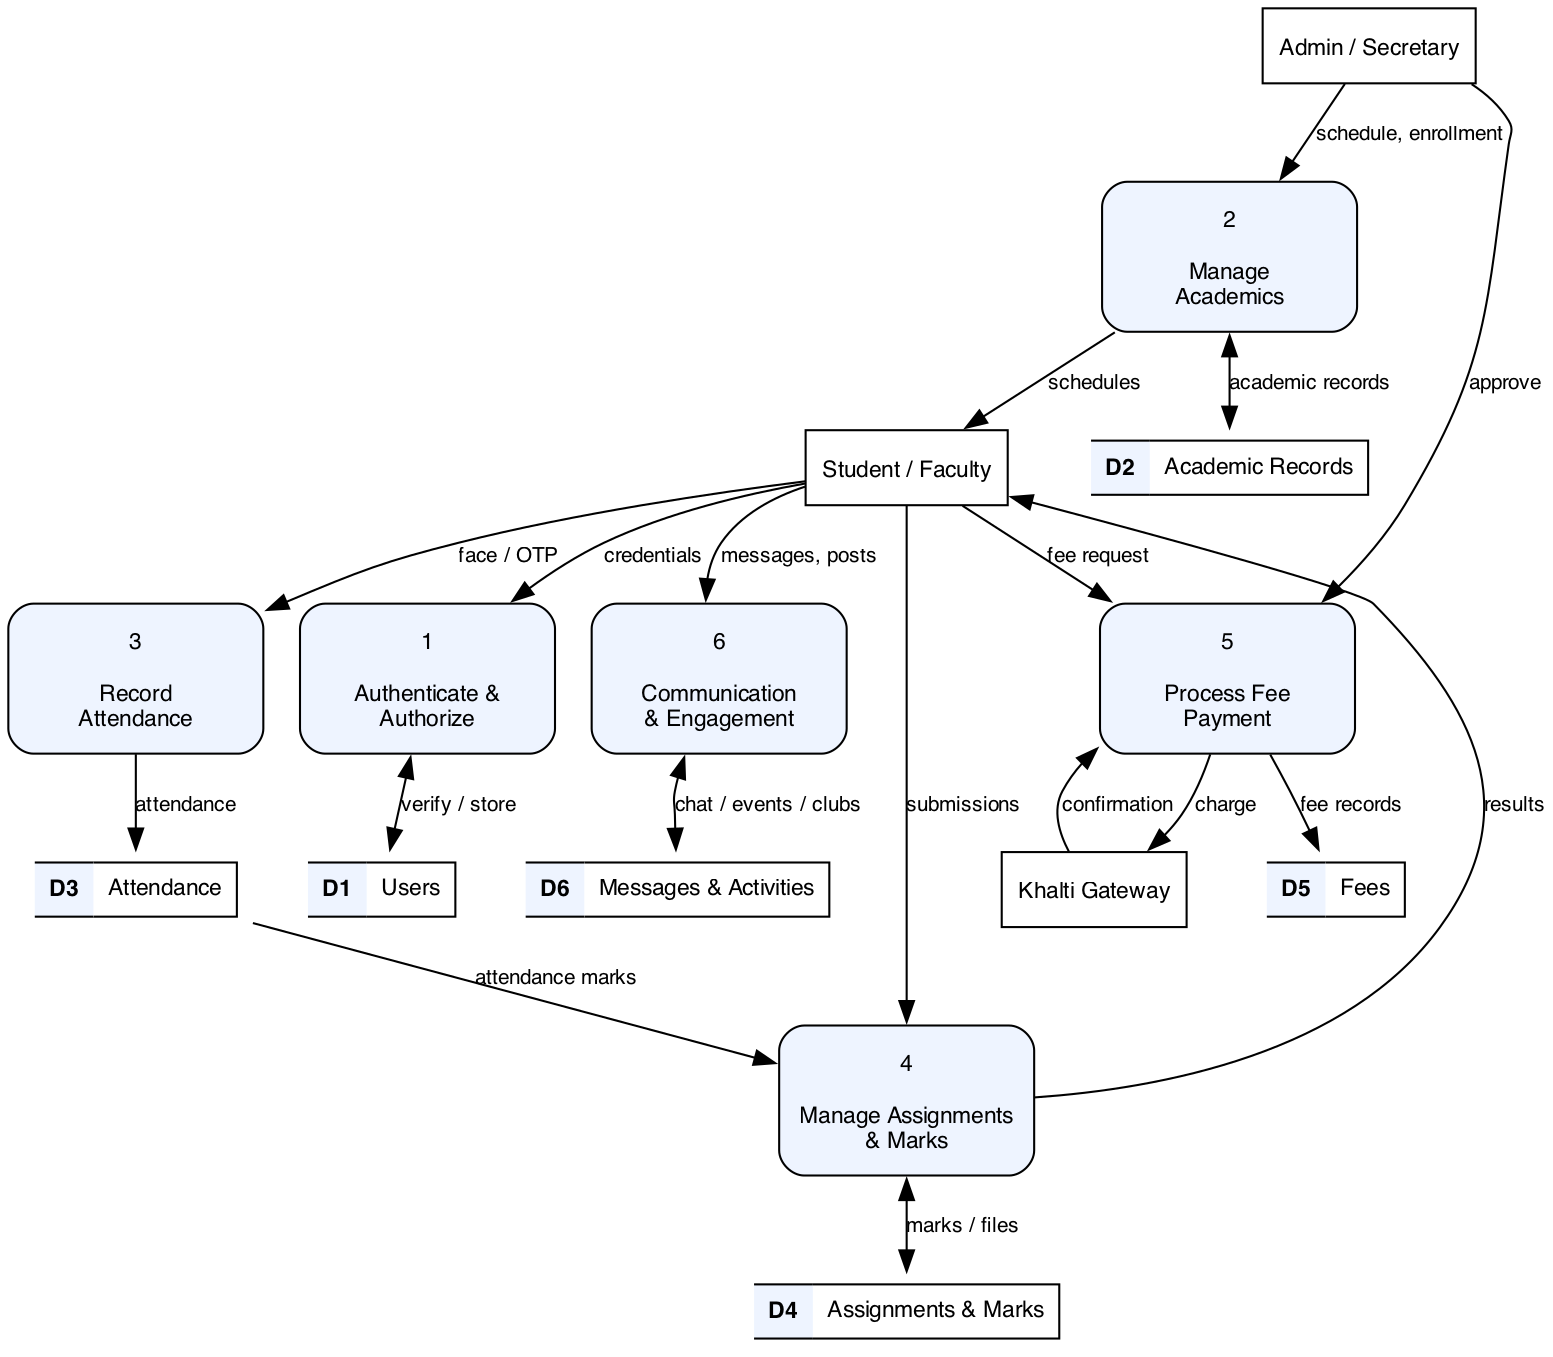
\includegraphics[width=0.92\textwidth,height=0.80\textheight,keepaspectratio]{figures/dfd_level1.png}
    \caption{Level 1 data flow diagram.}
    \label{fig:dfd1}
\end{figure}

\section{System Design}

\subsection{Architectural Design}

CampusEase follows a layered architecture. The presentation layer is an Angular single-page application running in the browser, with separate portals for students, faculty, and administrators and Highcharts-based dashboards. The application layer is a Node.js and Express REST API, complemented by a Socket.io server for real-time messaging, organized into route groups for authentication, academics, attendance, fees, and communication. The business logic layer contains the JWT authentication and role middleware, the face-recognition service, the internal-marks calculator, the payment handler, the email and one-time-password service, and the socket message hub. The data layer uses the Mongoose object-document mapper over a MongoDB database, and two external services, the Khalti payment gateway and an SMTP mail service, are integrated. Figure~\ref{fig:architecture} shows the overall architecture.

\begin{figure}[H]
    \centering
    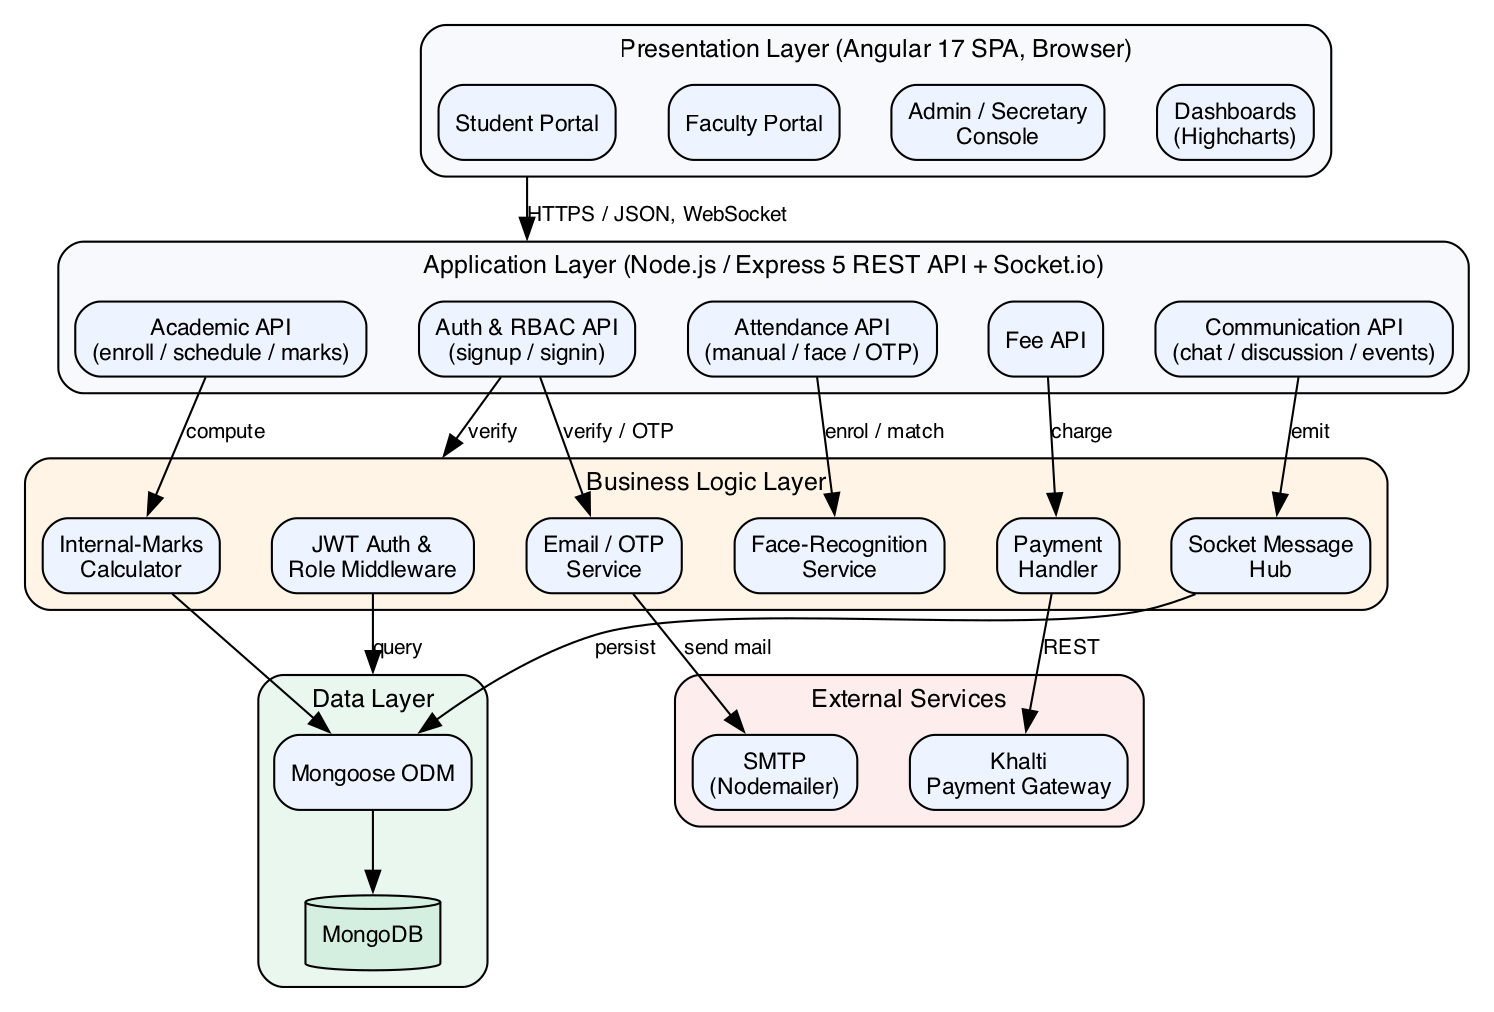
\includegraphics[width=0.98\textwidth,height=0.78\textheight,keepaspectratio]{figures/architecture.png}
    \caption{Layered system architecture of CampusEase.}
    \label{fig:architecture}
\end{figure}

\subsection{Database Schema Design}

The database is a set of MongoDB collections defined as Mongoose schemas. Table~\ref{tab:schema} summarizes the key collections and their purpose.

\begin{longtable}{|p{3.0cm}|p{4.4cm}|p{6.2cm}|}
\caption{Database schema summary (key collections).}
\label{tab:schema}\\
\hline
\textbf{Collection} & \textbf{Key Fields} & \textbf{Purpose} \\
\hline
\endfirsthead
\hline
\textbf{Collection} & \textbf{Key Fields} & \textbf{Purpose} \\
\hline
\endhead
User (register) & email (unique), name, rollno, password, role, department, isVerified & Stores all user accounts with their role and department for access control. \\
\hline
Enrollment\-Subjects & enrollment\_key, semester, department, subjects[] & Defines the subjects of a semester and the key students use to enroll. \\
\hline
Attendance / Face & email, rollno, subject, date, remarks; faceEncoding & Stores attendance records, including face-recognition enrollment data. \\
\hline
GiveAssignment / AnswerAssignment & subject, assignmentName, dueDate; rollno, assignmentFile, submitteddate & Stores assignments posted by faculty and submissions made by students. \\
\hline
MarksEntry / InternalMarks & studentId (FK), teacherId (FK), subjectName, marks; assignmentMarks, attendanceMarks & Stores entered marks and the computed internal marks. \\
\hline
Fee & studentId (FK), amount, method, status, receiptNumber & Stores fee payments and their approval status. \\
\hline
Message & sender (FK), receiver (FK), message, isRead, timestamp & Stores real-time chat messages between users. \\
\hline
\end{longtable}

\subsection{Interface Design (UI/UX)}

The user interface is organized into role-specific areas, designed for clarity and minimal training:

\begin{itemize}
    \item \textbf{Student portal:} enrollment, schedule, attendance, assignment submission, marks and academic records, fee payment, messaging, clubs, and events.
    \item \textbf{Faculty portal:} class scheduling, attendance, assignment posting and grading, marks entry, and model questions.
    \item \textbf{Admin / Secretary console:} user management, fee approval, department and enrollment-key management, ID cards, vacancies, sponsorships, and reports.
    \item \textbf{Dashboards:} summary statistics and charts, built with Highcharts, giving each role an at-a-glance overview.
\end{itemize}

\subsection{Activity Modelling}

Figure~\ref{fig:activity} shows the activity diagram for face-recognition attendance, one of the system's distinctive features. The student opens the attendance screen; if no face is registered yet, a face is captured and its encoding stored. A live face image is then captured and compared with the stored encoding. If the match confidence is high, attendance is marked present and persisted; otherwise the attempt is rejected and the student is prompted to retry.

\begin{figure}[H]
    \centering
    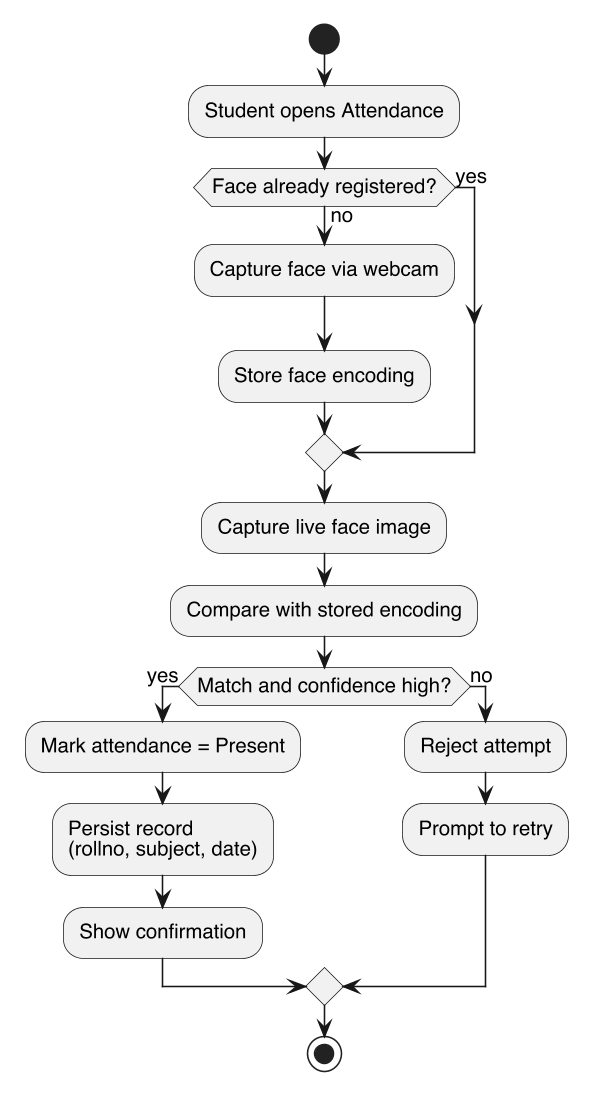
\includegraphics[width=0.65\textwidth,height=0.80\textheight,keepaspectratio]{figures/activity_diagram.png}
    \caption{Activity diagram for face-recognition attendance.}
    \label{fig:activity}
\end{figure}

\subsection{Sequence Modelling}

Figure~\ref{fig:sequence} shows the sequence diagram for online fee payment. The student initiates payment from the Angular application, which calls the Khalti gateway; on success the application posts the payment to the Express API, which records a fee with pending status and returns a receipt number. An administrator or finance officer later approves the payment, updating its status to paid.

\begin{figure}[H]
    \centering
    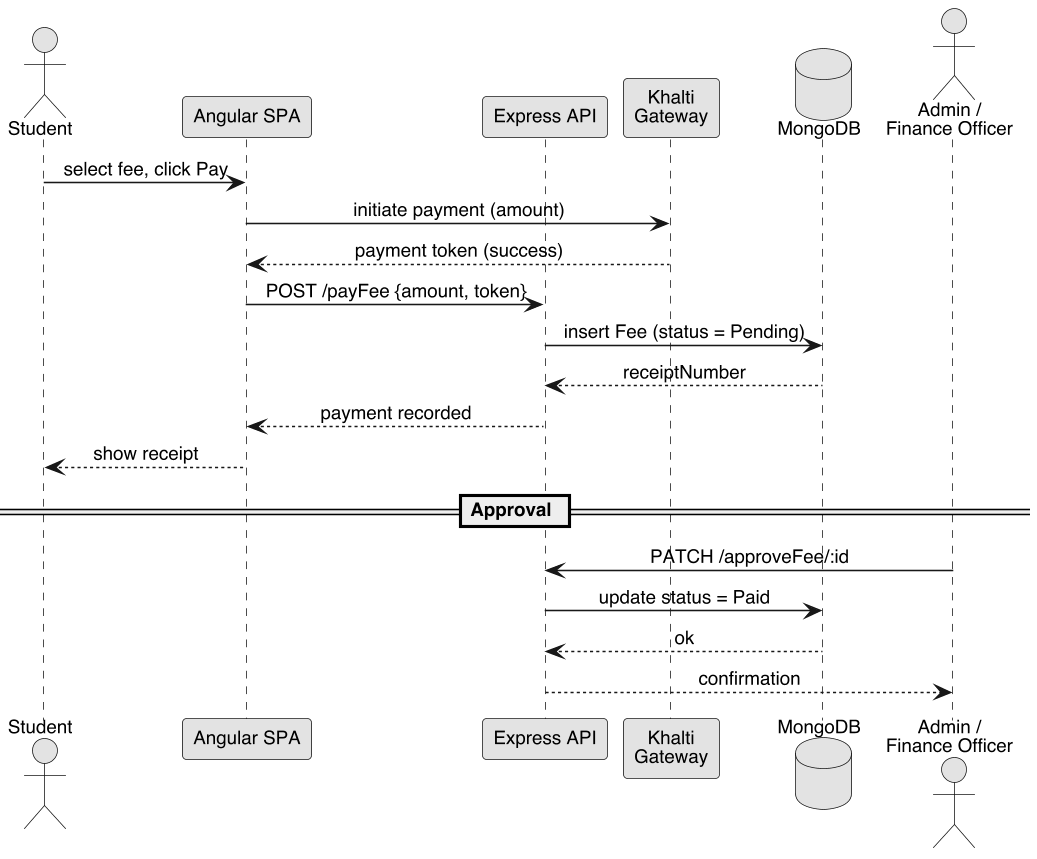
\includegraphics[width=0.95\textwidth,height=0.78\textheight,keepaspectratio]{figures/sequence_diagram.png}
    \caption{Sequence diagram for online fee payment.}
    \label{fig:sequence}
\end{figure}

% =====================================================================
% CHAPTER 4: IMPLEMENTATION AND TESTING
% =====================================================================
\chapter{Implementation and Testing}

\section{Implementation}

\subsection{Tools Used}

Development used Visual Studio Code as the editor, Node.js as the runtime, npm for package management, the Angular CLI for the frontend, MongoDB Compass for inspecting the database, and Git and GitHub for version control. Table~\ref{tab:techstack} lists the main technologies and the role each plays.

\begin{longtable}{|p{3.4cm}|p{10.1cm}|}
\caption{Technology stack used to build CampusEase.}
\label{tab:techstack}\\
\hline
\textbf{Technology} & \textbf{Role in CampusEase} \\
\hline
\endfirsthead
\hline
\textbf{Technology} & \textbf{Role in CampusEase} \\
\hline
\endhead
Angular & Single-page-application framework for the role-specific frontend portals~\cite{angular}. \\
\hline
TypeScript & Typed language used across the Angular frontend for safer, maintainable code. \\
\hline
Bootstrap \& ng-bootstrap & Responsive styling and ready-made UI components. \\
\hline
Node.js \& Express & JavaScript runtime and web framework providing the REST API~\cite{express}. \\
\hline
Socket.io & Real-time, bidirectional communication for messaging and presence~\cite{socketio}. \\
\hline
MongoDB & NoSQL document database for persistent storage~\cite{mongodb}. \\
\hline
Mongoose & Object-document mapper that defines schemas and queries MongoDB. \\
\hline
JSON Web Token & Stateless authentication tokens carried in the Authorization header. \\
\hline
bcrypt & One-way password hashing for stored credentials. \\
\hline
Multer & Middleware for handling file uploads (assignments, CVs, faces). \\
\hline
Nodemailer & Sends verification, one-time-password, and reset emails over SMTP. \\
\hline
Khalti & External payment gateway used for online fee payment~\cite{khalti}. \\
\hline
Highcharts & Charting library used for dashboards and reports. \\
\hline
\end{longtable}

\subsection{Implementation Details of Modules}

\textbf{Authentication and Role Module.}
This module handles registration, email verification, login, and password management. Passwords are hashed with bcrypt and never stored in plain text. On login the server issues a JSON Web Token, which the client sends with every subsequent request. Middleware verifies the token and checks the user's role and department against the roles permitted for each endpoint, enforcing role-based access control across the system.

\textbf{Academic Module.}
The academic module covers subject enrollment, class scheduling, and academic records. A student enrolls in a semester's subjects using an enrollment key; faculty and staff create and maintain class schedules; and academic records and transcripts are stored and retrieved per student.

\textbf{Attendance Module.}
Attendance can be recorded in three ways. Manual entry lets faculty mark a class roll directly. One-time-password attendance issues a short-lived code that students enter to confirm presence. Face-recognition attendance captures a student's face through the webcam, stores an encoding on first registration, and on later attempts matches a live capture against the stored encoding before marking the student present.

\textbf{Assignments and Marks Module.}
Faculty post assignments with a due date and an optional file; students submit answers with file uploads. Faculty enter marks for each student and subject, and the internal-marks calculator combines assignment marks and attendance marks into a computed internal score, removing a tedious manual calculation.

\textbf{Fee Payment Module.}
Students pay fees online through the Khalti gateway. The frontend initiates the payment, and on success the backend records a fee with a receipt number and a pending status. An administrator or finance officer then approves or rejects the payment, and the status is updated accordingly. Payments by other methods are recorded and approved manually.

\textbf{Communication and Engagement Module.}
Real-time one-to-one messaging is implemented with Socket.io: each connected user registers their socket, online presence is tracked, and messages are delivered instantly to the recipient and persisted to MongoDB. Discussion forums, events, and club membership round out the engagement features.

\textbf{Administration and Career Module.}
Authorized staff manage users, departments, and enrollment keys, approve fees and ID-card requests, and post job vacancies. Students submit CVs and sponsorship requests and generate digital ID cards. Dashboards built with Highcharts summarize activity for each role.

\section{Testing}

Because CampusEase is built module by module, testing was carried out module by module and then end to end. Each feature was tested with representative inputs as it was completed, and the integrated system was exercised through the user interface for each role.

\subsection{Test Cases for Unit Testing}

\begin{longtable}{|p{1.2cm}|p{4.6cm}|p{4.8cm}|p{1.8cm}|}
\caption{Unit test cases.}
\label{tab:unittest}\\
\hline
\textbf{ID} & \textbf{Test Case} & \textbf{Expected Result} & \textbf{Status} \\
\hline
\endfirsthead
\hline
\textbf{ID} & \textbf{Test Case} & \textbf{Expected Result} & \textbf{Status} \\
\hline
\endhead
UT-01 & Register with a new email & Account created, verification email sent & Pass \\
\hline
UT-02 & Register with an existing email & Registration rejected with a clear message & Pass \\
\hline
UT-03 & Hash and verify password & Correct password verifies, incorrect one does not & Pass \\
\hline
UT-04 & Issue and verify JWT & Valid token is accepted, tampered token is rejected & Pass \\
\hline
UT-05 & Role check on a protected route & A role without permission is denied access & Pass \\
\hline
UT-06 & Enroll using a valid enrollment key & Student enrolled in the semester's subjects & Pass \\
\hline
UT-07 & Mark manual attendance & Attendance record stored with correct fields & Pass \\
\hline
UT-08 & Face-recognition match & A matching face marks attendance present & Pass \\
\hline
UT-09 & Submit an assignment file & Submission stored with student and subject & Pass \\
\hline
UT-10 & Calculate internal marks & Assignment and attendance marks combine correctly & Pass \\
\hline
UT-11 & Record a fee payment & Fee stored with pending status and receipt number & Pass \\
\hline
UT-12 & Approve a fee payment & Fee status updates to paid & Pass \\
\hline
UT-13 & Send a real-time message & Message delivered to recipient and persisted & Pass \\
\hline
UT-14 & Generate a digital ID card & ID card created for an approved request & Pass \\
\hline
\end{longtable}

\subsection{Test Cases for System Testing}

\begin{longtable}{|p{1.2cm}|p{4.8cm}|p{5.6cm}|p{1.6cm}|}
\caption{System (end-to-end) test cases.}
\label{tab:systest}\\
\hline
\textbf{ID} & \textbf{Test Case} & \textbf{Expected Result} & \textbf{Status} \\
\hline
\endfirsthead
\hline
\textbf{ID} & \textbf{Test Case} & \textbf{Expected Result} & \textbf{Status} \\
\hline
\endhead
ST-01 & Register, verify, and log in as a student & Student reaches the student portal & Pass \\
\hline
ST-02 & Log in with wrong credentials & Login rejected with a clear message & Pass \\
\hline
ST-03 & Enroll in subjects and view schedule & Subjects and schedule shown correctly & Pass \\
\hline
ST-04 & Take attendance by face and by OTP & Both methods record attendance & Pass \\
\hline
ST-05 & Post and submit an assignment & Faculty posts, student submits, file stored & Pass \\
\hline
ST-06 & Enter marks and view internal marks & Marks entered, internal marks computed & Pass \\
\hline
ST-07 & Pay a fee online and approve it & Payment recorded, then approved by staff & Pass \\
\hline
ST-08 & Send messages between two users & Messages delivered in real time & Pass \\
\hline
ST-09 & Manage users as an administrator & Create, update, and delete users work & Pass \\
\hline
ST-10 & Role-based access enforcement & Each role can access only permitted areas & Pass \\
\hline
ST-11 & Post a vacancy and submit a CV & Vacancy listed, CV stored and listed & Pass \\
\hline
ST-12 & View dashboard charts & Charts render with correct summary data & Pass \\
\hline
\end{longtable}

\subsection{Results and Discussion}

All unit and system test cases passed. Registration, email verification, and login behaved correctly, and the JSON-Web-Token and role checks reliably allowed permitted actions while rejecting unauthorized ones. The academic modules worked end to end: students enrolled with a key, attendance was recorded by all three methods, assignments were posted and submitted, and internal marks were computed correctly from assignment and attendance scores. Online fee payment recorded a pending fee that staff could approve, and real-time messaging delivered messages instantly while persisting them for later retrieval. The administrative features, user management, vacancies, CV submission, ID cards, and dashboards, all functioned as expected. The main observation is that building the role model and shared data model first paid off: because every later module relied on them, getting authentication and access control right early made the remaining modules straightforward to add and test. The overall control and data flow of the system is summarized in the flowchart in Figure~\ref{fig:flowchart}.

\begin{figure}[H]
    \centering
    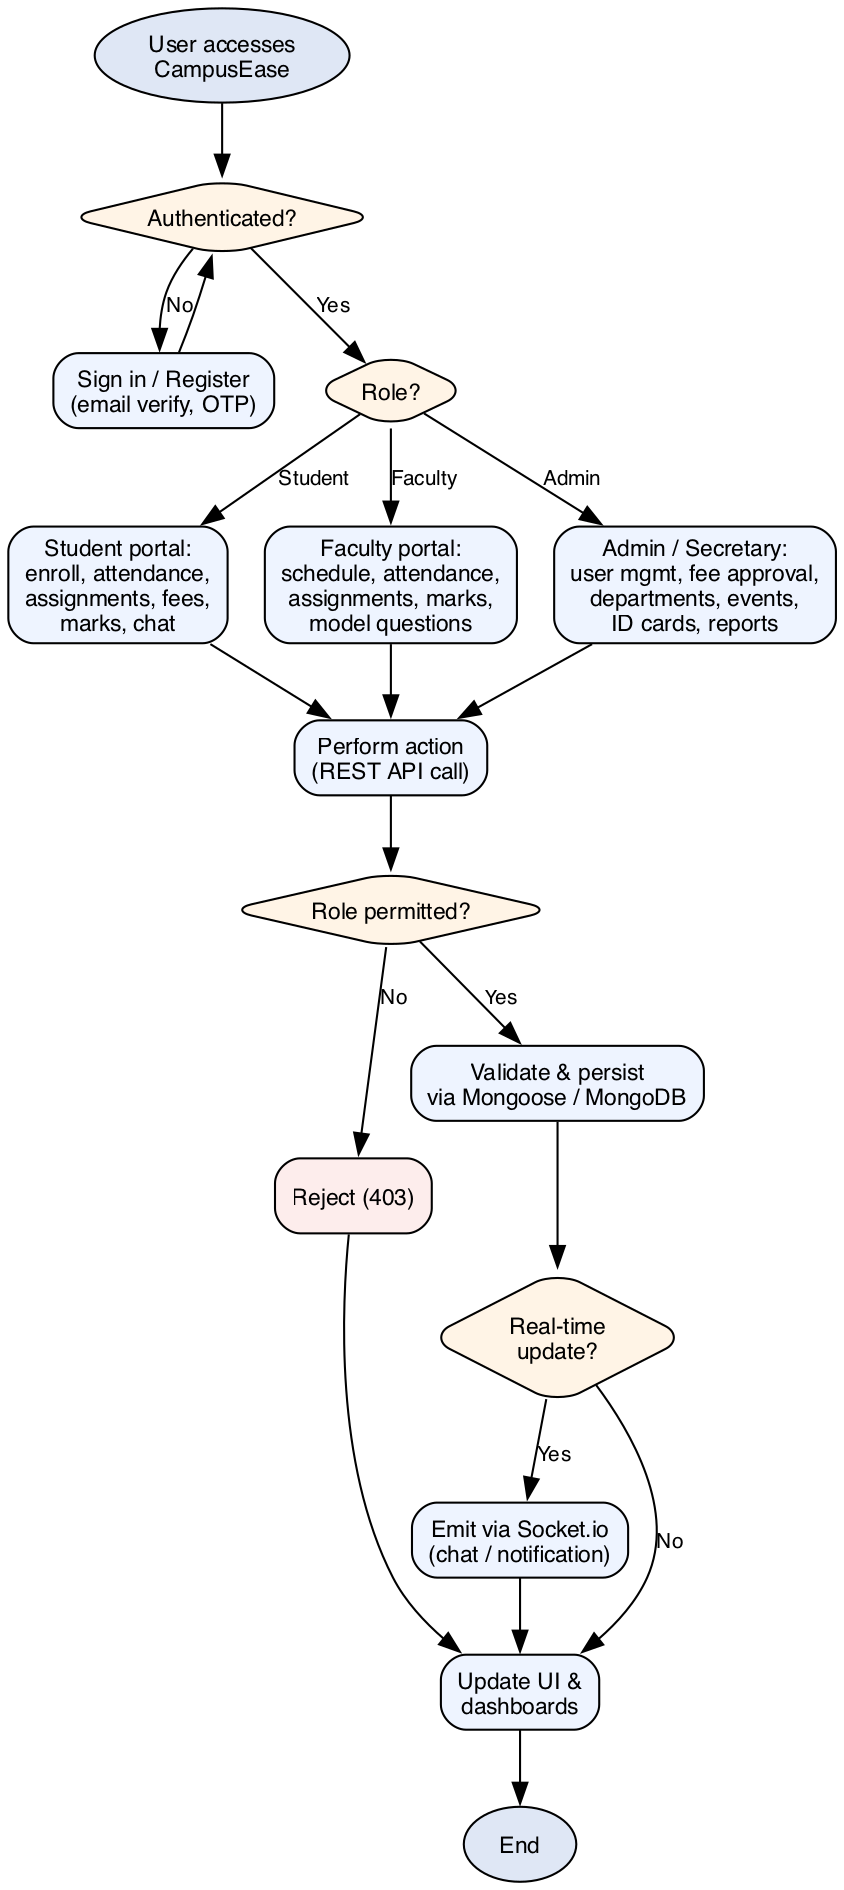
\includegraphics[width=0.62\textwidth,height=0.82\textheight,keepaspectratio]{figures/flowchart.png}
    \caption{System flowchart of CampusEase.}
    \label{fig:flowchart}
\end{figure}

% =====================================================================
% CHAPTER 5: CONCLUSION AND FUTURE RECOMMENDATIONS
% =====================================================================
\chapter{Conclusion and Future Recommendations}

\section{Conclusion}

This project set out to replace the manual, fragmented processes of a college with a single, integrated, role-aware web platform, and it achieves that goal. CampusEase is a complete, working application that unifies authentication and role-based access, subject enrollment and scheduling, attendance by manual, one-time-password, and face-recognition methods, assignment distribution and submission, marks entry and automatic internal-marks calculation, online fee payment with administrative approval, and real-time communication through messaging, discussions, events, and clubs, along with career services, sponsorship, and digital ID cards. Built with an Angular frontend, a Node.js and Express API with Socket.io, and MongoDB through Mongoose, secured with JSON Web Tokens and bcrypt, the system reduces administrative workload, minimizes errors, and improves transparency and communication. Every objective set out in Chapter~1 was met, and testing confirmed that each module and the system as a whole behave correctly.

\section{Lesson Learnt / Outcome}

The project reinforced several lessons. First, designing the role-based access model and the shared user data model before the feature modules paid off, because almost every later feature depended on them. Second, an iterative, module-by-module approach made a large, multi-feature system manageable and allowed continuous integration and testing. Third, integrating external services such as the Khalti payment gateway and an email provider showed the importance of handling failures gracefully so that the rest of the system keeps working. The outcome is a deployable, multi-role college automation platform together with practical experience in full-stack web development, real-time systems, secure authentication, and third-party integration.

\section{Future Recommendations}

Several enhancements would extend the system beyond its current scope:

\begin{itemize}
    \item \textbf{Mobile application} for students and faculty, reusing the existing API, for fully on-the-go access.
    \item \textbf{Push and email notifications} for high-priority events such as new marks, fee due dates, and announcements.
    \item \textbf{Advanced analytics} on attendance, performance, and fee collection to support data-driven decisions.
    \item \textbf{Production-grade security} with refresh-token rotation, centralized session management, and rate limiting.
    \item \textbf{Scalable deployment} with a replicated MongoDB cluster and horizontal scaling of the API for multi-campus use.
    \item \textbf{More payment options} and automatic reconciliation alongside the existing Khalti integration.
\end{itemize}

% =====================================================================
% APPENDICES
% =====================================================================
\clearpage
\chapter*{Appendices}
\addcontentsline{toc}{chapter}{Appendices}

\section*{Appendix A: Application Screenshots}

\renewcommand{\thefigure}{A.\arabic{figure}}
\setcounter{figure}{0}

The following screenshots show the running CampusEase application.

\begin{figure}[H]
    \centering
    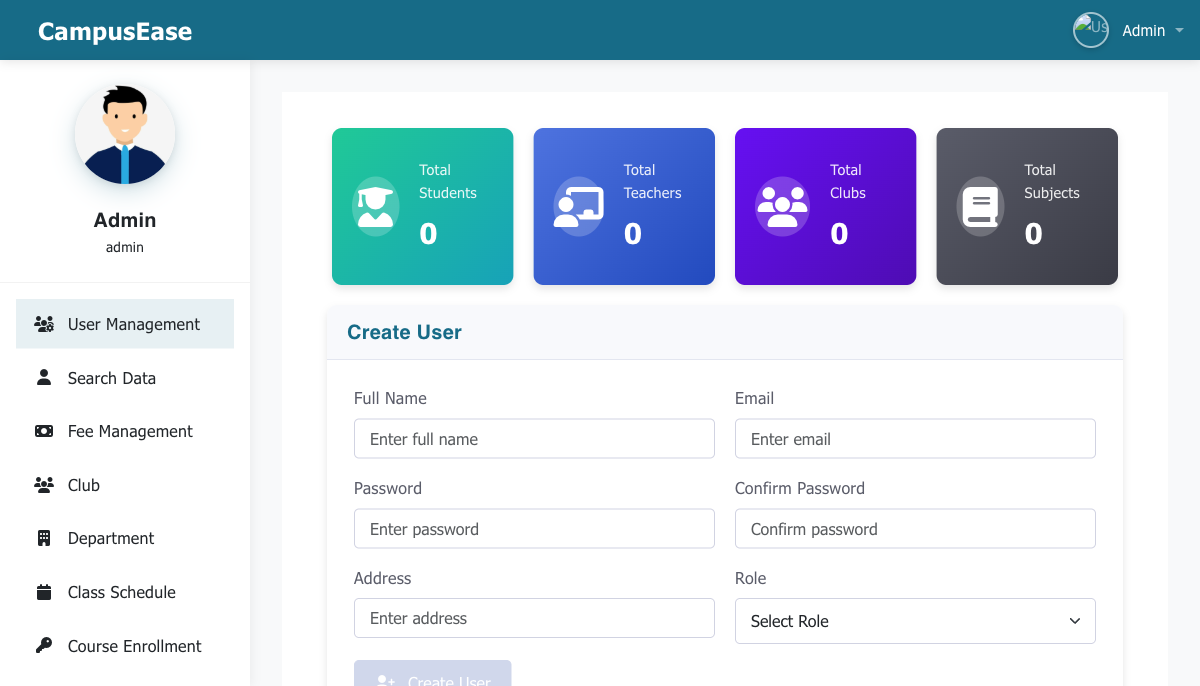
\includegraphics[width=0.95\textwidth]{figures/app_admin_dashboard.png}
    \caption{Administrator console: summary cards and the create-user panel (empty institution).}
\end{figure}

\begin{figure}[H]
    \centering
    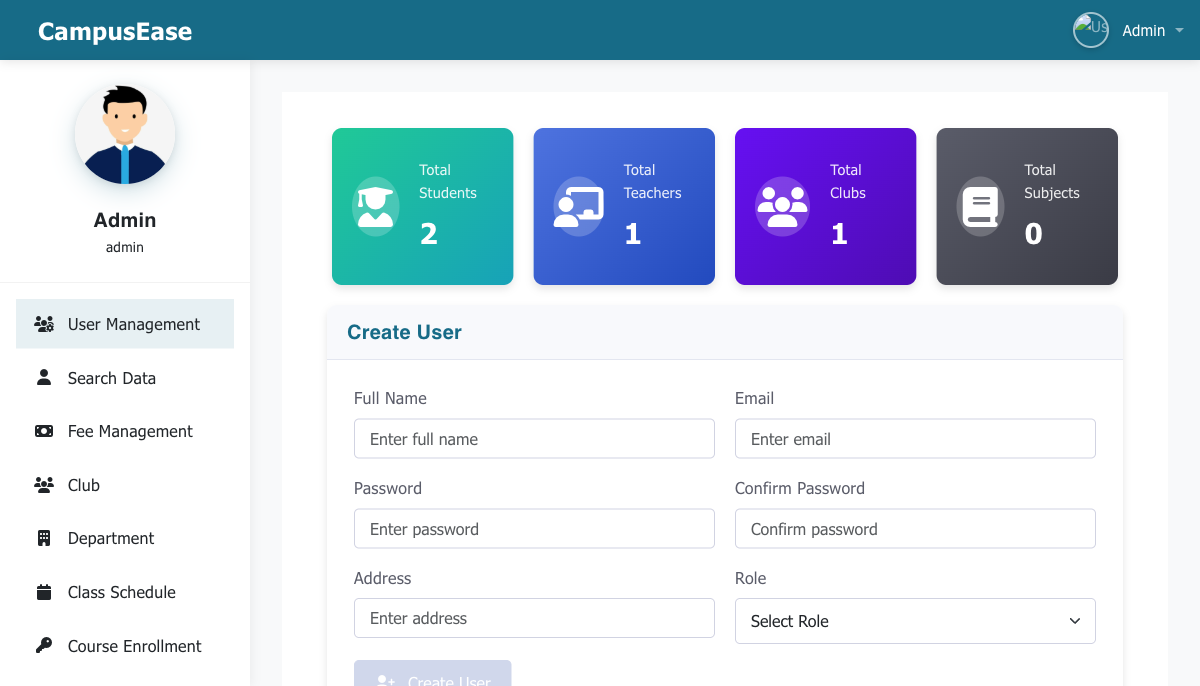
\includegraphics[width=0.95\textwidth]{figures/app_user_management.png}
    \caption{User-management screen with populated student, teacher, and club counts.}
\end{figure}

\section*{Appendix B: Representative Source Code}

The role-based access control middleware that protects the API is reproduced below.

\begin{lstlisting}[language=Java]
const jwt = require("jsonwebtoken");

// Verify the JSON Web Token sent in the Authorization header
function verifyToken(req, res, next) {
  const header = req.headers["authorization"] || "";
  const token = header.startsWith("Bearer ") ? header.slice(7) : header;
  if (!token) return res.status(401).json({ message: "No token provided" });
  try {
    req.user = jwt.verify(token, process.env.JWT_SECRET);
    next();
  } catch (e) {
    return res.status(401).json({ message: "Invalid or expired token" });
  }
}

// Allow the request only if the user's role is in the allowed list
function verifyRole(allowedRoles) {
  return (req, res, next) => {
    if (!req.user || !allowedRoles.includes(req.user.role)) {
      return res.status(403).json({ message: "Access denied" });
    }
    next();
  };
}

module.exports = { verifyToken, verifyRole };
\end{lstlisting}

\clearpage
\addcontentsline{toc}{section}{Appendix C: Project Log Book}

\newcommand{\logsheetpage}[1]{%
\thispagestyle{plain}\begingroup\singlespacing\setlength{\parskip}{0pt}%
\begin{center}\textbf{\fontsize{14}{17}\selectfont Project Log Book Entry Sheet}\end{center}
\vspace{0.3cm}
\noindent\begin{minipage}[t]{0.52\textwidth}Meeting No.: \dotfill\end{minipage}\hfill\begin{minipage}[t]{0.42\textwidth}Date: \dotfill\end{minipage}\par
\vspace{12pt}\noindent\begin{minipage}[t]{0.52\textwidth}Start Time: \dotfill\end{minipage}\hfill\begin{minipage}[t]{0.42\textwidth}Finish Time: \dotfill\end{minipage}\par
\vspace{16pt}\noindent\textbf{Discussion Topics:}\par
\vspace{8pt}1.~\dotfill\par\vspace{10pt}2.~\dotfill\par\vspace{10pt}3.~\dotfill\par\vspace{10pt}4.~\dotfill\par
\vspace{14pt}\noindent\textbf{Achievements:}\par
\vspace{8pt}1.~\dotfill\par\vspace{10pt}2.~\dotfill\par\vspace{10pt}3.~\dotfill\par\vspace{10pt}4.~\dotfill\par
\vspace{14pt}\noindent\textbf{Problems (if any):}\par
\vspace{8pt}1.~\dotfill\par\vspace{10pt}2.~\dotfill\par\vspace{10pt}3.~\dotfill\par\vspace{10pt}4.~\dotfill\par
\vspace{14pt}\noindent\textbf{Task for next meeting:}\par
\vspace{8pt}1.~\dotfill\par\vspace{10pt}2.~\dotfill\par\vspace{10pt}3.~\dotfill\par\vspace{10pt}4.~\dotfill\par
\vspace{16pt}\noindent\rule{\textwidth}{0.4pt}\par
\vspace{8pt}\noindent\begin{minipage}[t]{0.55\textwidth}Student Name: #1\\[16pt]Signature: \dotfill\end{minipage}\hfill\begin{minipage}[t]{0.4\textwidth}\centering Mentor Signature\\[22pt]\dotfill\end{minipage}\par
\endgroup\clearpage}

\logsheetpage{Bhupendra Malla}
\logsheetpage{Bhupendra Malla}
\logsheetpage{Bhupendra Malla}
\logsheetpage{Bhupendra Malla}
\logsheetpage{Bhupendra Malla}

% =====================================================================
% REFERENCES (IEEE)
% =====================================================================
\clearpage
\addcontentsline{toc}{chapter}{References}
\begin{thebibliography}{99}

\bibitem{angular} Google, ``Angular Documentation,'' 2025. [Online]. Available: \url{https://angular.dev/}

\bibitem{express} OpenJS Foundation, ``Express Web Framework Documentation,'' 2025. [Online]. Available: \url{https://expressjs.com/}

\bibitem{nodejs} OpenJS Foundation, ``Node.js Documentation,'' 2025. [Online]. Available: \url{https://nodejs.org/en/docs}

\bibitem{mongodb} MongoDB Inc., ``MongoDB Manual,'' 2025. [Online]. Available: \url{https://www.mongodb.com/docs/}

\bibitem{socketio} Socket.io, ``Socket.io Documentation,'' 2025. [Online]. Available: \url{https://socket.io/docs/v4/}

\bibitem{khalti} Khalti, ``Khalti Payment Gateway Documentation,'' 2025. [Online]. Available: \url{https://docs.khalti.com/}

\bibitem{moodle} Moodle Pty Ltd., ``Moodle Documentation,'' 2025. [Online]. Available: \url{https://docs.moodle.org/}

\bibitem{googleclassroom} Google, ``Google Classroom Help,'' 2025. [Online]. Available: \url{https://support.google.com/edu/classroom/}

\bibitem{jwt} Internet Engineering Task Force, ``RFC 7519: JSON Web Token (JWT),'' 2015. [Online]. Available: \url{https://www.rfc-editor.org/rfc/rfc7519}

\bibitem{beck2001} K. Beck et al., ``Manifesto for Agile Software Development,'' 2001. [Online]. Available: \url{https://agilemanifesto.org/}

\end{thebibliography}

\end{document}
